%% LyX 2.0.4 created this file.  For more info, see http://www.lyx.org/.
%% Do not edit unless you really know what you are doing.
\documentclass[english]{article}
\usepackage[T1]{fontenc}
\usepackage[latin9]{inputenc}
\usepackage[a4paper]{geometry}
\geometry{verbose,tmargin=1cm,bmargin=2cm,lmargin=1cm,rmargin=1cm}
\setlength{\parskip}{\medskipamount}
\setlength{\parindent}{0pt}
\usepackage{graphicx}
\graphicspath{{Figures/}}

\usepackage{babel}
\begin{document}

\title{Opstelling simulatie HiSPARC detector}


\author{N.G. Schultheiss}

\maketitle

\section*{Benodigdheden}

\noindent \begin{center}
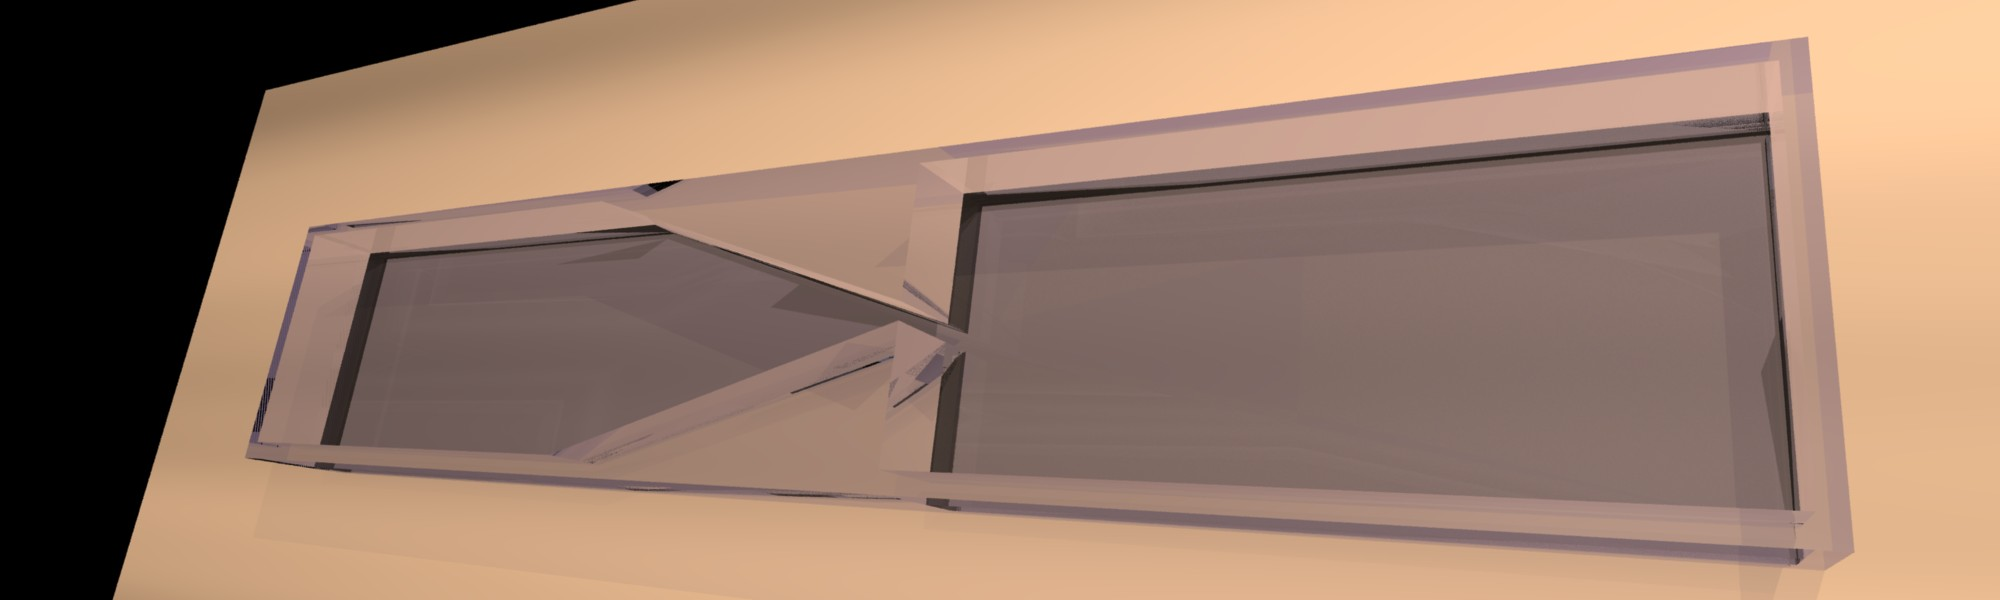
\includegraphics[width=16cm]{simulatie4}
\par\end{center}

De opstelling is samen te stellen door de volgende onderdelen aan
elkaar te lijmen:
\begin{itemize}
\item Bodemplaat 1{*} perspex 500mm{*}80mm{*}3mm of 500mm{*}80mm{*}5mm
\item Zijplaat 2{*} perspex 500mm{*}53mm{*}3mm of 500mm{*}55mm{*}5mm
\item Kopplaat 2{*} perspex 86mm{*}53mm{*}3mm of 90mm{*}55mm{*}5mm
\end{itemize}
In deze bak zijn twee driehoekige perspex blokken geplaatst. Hiervan
zijn de maten in figuur 2 te vinden.

\newpage{}

\begin{figure}
\begin{centering}
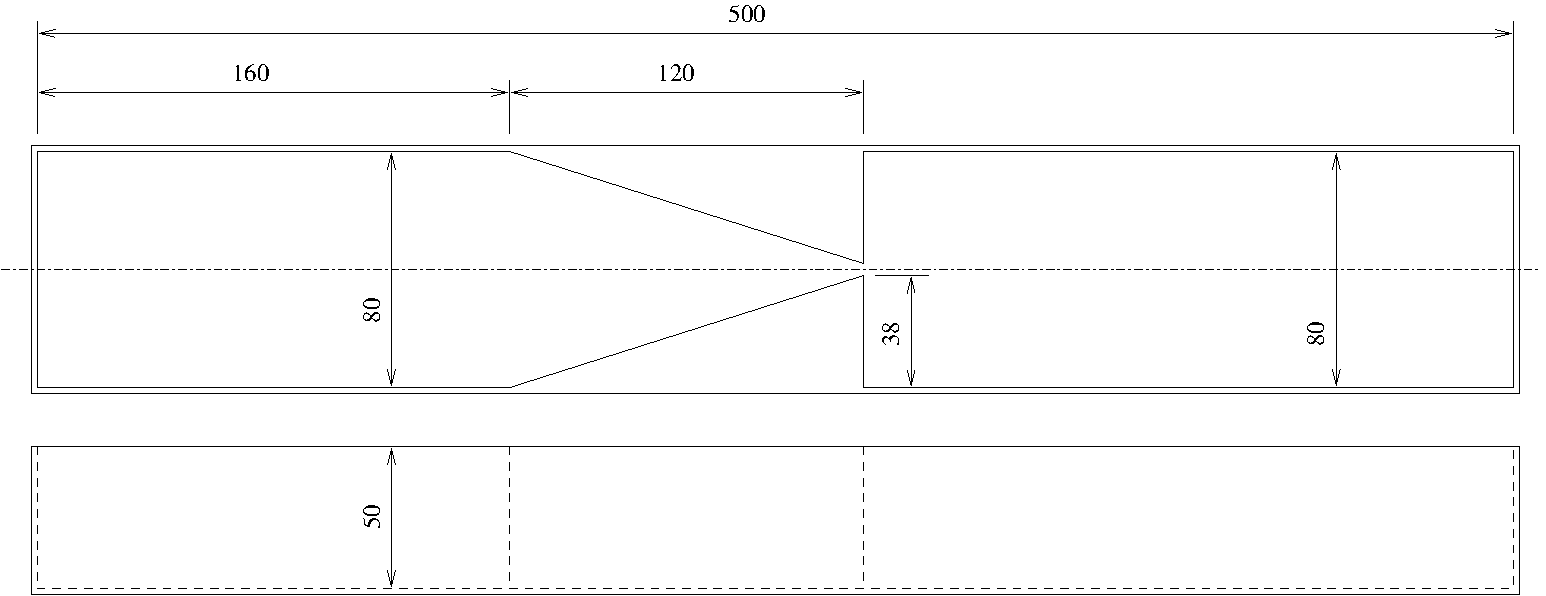
\includegraphics[angle=90,scale=0.75]{bak-maat}
\par\end{centering}

\caption{Samenstelling}


\end{figure}


\newpage{}

\begin{figure}
\noindent \begin{centering}
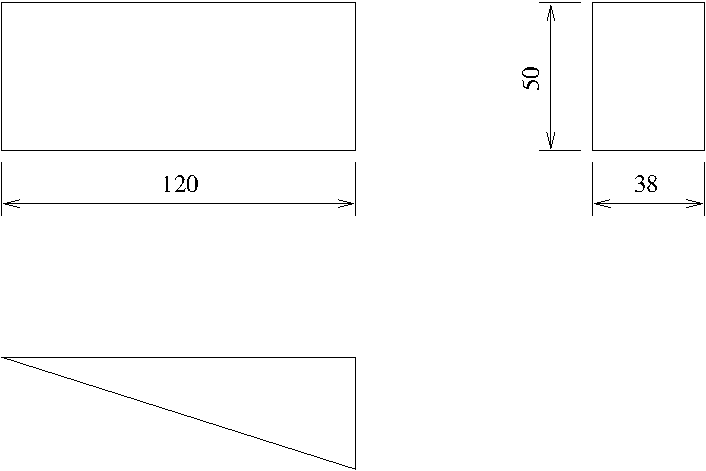
\includegraphics[scale=0.75]{blok}
\par\end{centering}

\caption{Afmetingen van het blok}


\end{figure}

\end{document}
